This chapter will discuss the evaluation process of the application including testing, evaluation experiments, and, the results gathered.

\section{Testing}
Application testing was performed during, and, after the implementation process of this project. Testing is vitally important in software development to ensure code is bug free, and, ready for deployment.

\subsection{User Testing}
While the application was being developed, new features were consistently tested by having the application run locally, then experimenting with the new features created. Potential users were recruited throughout to test the application and provide feedback. This technique provided invaluable feedback, and, testing of the application, helping to create a more robust, and, enjoyable user experience.

\subsection{Jest Testing}
Jest is a testing framework that allows the easy creation of tests for JavaScript code. Jest was used to create unit, and snapshot tests for this project. Unit testing is where individual 'units' of an application are tested independently, this method was used to test functions, and, expected behaviour of the application. 

\begin{figure}[!htbp]
    \centering
    \begin{subfigure}[b]{0.8\textwidth}
        \begin{lstlisting}[language=jsJsx]
        test("correct conversion", () => {
          expect(polarToCart(0, 0, 5, 90)).toStrictEqual({ x: 5, y: 0 });
        });
        test("navigation to home", () => {
            fireEvent.press(screen.getByTestId("pressableIcon"));
            expect(navigation.navigate).toBeCalledWith("HomeScreen");
        });
        \end{lstlisting}
    \end{subfigure}
\caption[Example of a unit test]{Example of a unit test on a function converting polar coordinates, to Cartesian, and, navigation.}
\label{fig:jestUnit}
\end{figure}
\FloatBarrier

Here we can see a test is created that expects a certain return value from the \texttt{polarToCart} function, this will either pass or fail depending on this value. Unit tests were also used to test aspects such as navigation, as seen above we are expecting the navigate function to be called with a parameter of "HomeScreen" when the \texttt{pressableIcon} has been pressed. These tests were used throughout the process of testing the components, and, screens of the application. Jest also provides support for snapshot testing, this is a method used to test that the user interface has not unexpectedly changed. 

\begin{figure}[!htbp]
    \centering
    \begin{subfigure}[b]{0.8\textwidth}
        \begin{lstlisting}[language=jsJsx]
        test("Check GroupScreen loading correctly", async () => {
          const domTree = renderer
            .create(<GroupScreen/>)
            .toJSON();
          expect(domTree).toMatchSnapshot();
        });
        \end{lstlisting}
    \end{subfigure}
\caption{Example of a snapshot test on the GroupScreen}
\label{fig:jestSnap}
\end{figure}
\FloatBarrier

Here a snapshot test is created to check the user interface is loading correctly for the \texttt{GroupScreen}. The first time a snapshot test is run Jest creates, and, stores a JSON snapshot of the user interface. When run again, this snapshot is then compared against the current user interface for differences, failing if the two snapshots differ. All tests for the application were executed through an \texttt{npm test} command, and, on commits to the main, and, test branches from a GitHub action \ref{ghActions}.

\subsection{Testing Challenges}\label{testChall}

The main challenge that presented itself during testing was application code relying on Firebase. As all screens contained application, and, user interface code this meant these elements could not be separately tested as the user interface relied on this application code. Many solutions were investigated but unfortunately none were suitable within the time constraints of the  project. To be able to fully test this application, a Firebase local emulator suite would have to be set up to run tests locally. To learn and set up this emulator suite along with writing these tests was not feasible, but is a feature that would be great to integrate in future releases for greater test coverage. The alternative was to mock all the Firebase functions, and, services that were used to provide mocked inputs to the  user interface, and application functions, unfortunately this was also infeasible within the time constraints. Due to this, full test coverage was not able to be achieved for all screens, however, components were unaffected so an average of 84.31\% of the lines of component code were covered by tests. The user interface of screens was also tested with snapshot, and, unit testing establishing some test coverage.   


\section{Experiment}
To evaluate the application an experiment was planned to gather user feedback, and, measure usability. The initial plan was to have participants download the application, then complete the experiment. However, it was discovered that if the user was using an iOS device, they could not simply access a link and download the application. Apple's TestFlight platform is designed to alleviate this struggle by allowing developers to upload builds and have users download the application from there, this however is part of Apple's developer program, a paid service, so was not suitable. It was decided at this stage that two similar experiments were to be run, one in person on a device with the application installed, and, an online survey showcasing application screenshots and recordings. This approach was taken to ensure there was a sufficient number of participants in the evaluation due to the in person experiment being run solely on one device, hampering the ability to gather responses. 

\subsection*{Ethics}
Both experiments were performed in line with the University of Glasgow's School of Computer Science ethics checklist \cite{ethics}. All participants consented, were allowed to ask any questions, and, were provided with contact details. A brief, and, debrief were provided to all participants stating the aims of the experiment, and, reminding the participant they are free to stop at any time.

\subsection*{Participants}
A wide variety of ages, genders, and technological backgrounds were consulted in this evaluation. The majority of the participants were part of the target demographic for the application, aged eighteen to thirty. 

\subsection{In Person}
The goals of the in person evaluation were to measure the usability of application, and, gather user feedback on their experience. The participant was first presented with some introductory questions to gain some initial opinions on the problem this application aims to solve, usage of similar concepts, and, the concept of this application (see\ref{appendix:introQns}).
Evaluating usability comprised of the participant completing a set of tasks, after each task the participant was asked the single ease question \cite{seq}, \textit{How difficult did you find this task?}. This was answered through a five point Likert scale ranging from very difficult, to very easy. The tasks were designed to incorporate all key areas of the application, creating accounts and groups, adding friends, and, customizing the user experience (see \ref{appendix:tasks}). This was further complemented by the use of the system usability scale (SUS) \cite{sus}, the industry standard for evaluating usability of products. The SUS comprises of ten questions answered through a five point Likert scale ranging from strongly disagree, to strongly agree (see \ref{appendix:susQns}). This was completed by the participant after all the tasks. Upon completion the participant was asked some concluding questions used to gather user feedback after usage of the application (see \ref{appendix:concludQns}). 
For an example survey response see \cite{evalRespWApp}.

\subsection{Online}
The online evaluation consisted of the same introductory, and, concluding questions but with a change to the usability evaluation. As the user would not have direct interaction with the application, the usability study performed during the in person evaluation was not suitable. Instead, two screen recordings of an example user interacting with the application were created, evaluated through Likert scale questions regarding the video content (see \ref{appendix:vidQns}). The participant was then asked to answer some general questions regarding the application and were given several screenshots of the application for reference (see \ref{appendix:onlineGenQns}). Although it was not possible to use the system usability scale, questions were designed to be very similar to gather meaningful results. For an example survey response see \cite{evalRespNoApp}. 

\section{Results}
In total there were 32 participants in the experiment, 24 online, and, 8 in person. The combination of both an in person, and, online evaluation allowed the gathering of a suitable number of responses which would not have been possible with a purely in person evaluation.

\subsection{Introductory \& Concluding Questions}
The responses to the introductory, and, concluding questions have been combined and presented below. The results from the introductory questions \ref{fig:introAns}, confirm that people do have issues with planning activities due to being unaware of their status, the problem this application aims to solve. Participants show a clear interest in the application concept with 91\% being likely to use an app to graphically see their friends status. 

\begin{figure}[H]

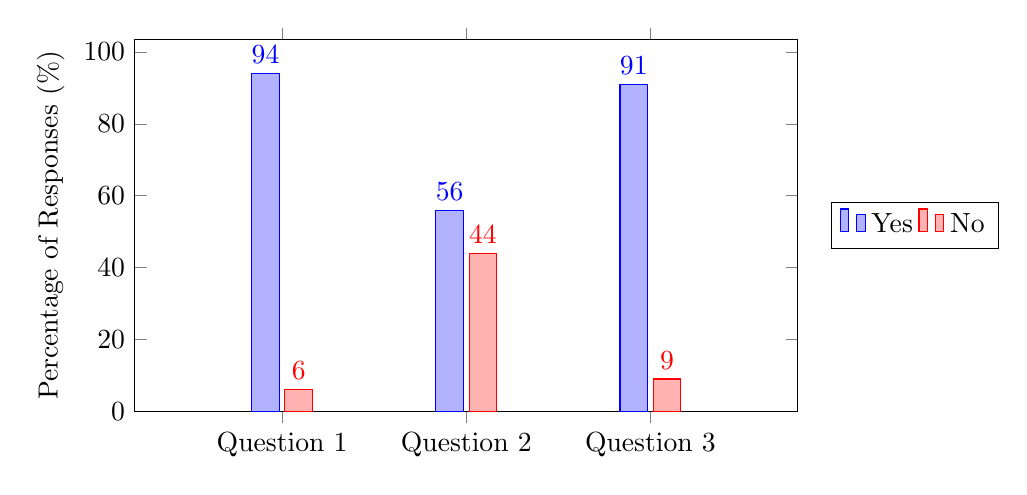
\begin{tikzpicture}  
\begin{axis}  
[  
    ybar,
    width=10cm,
    height=6.3cm,
    enlarge x limits=0.4,     
    ylabel={Percentage of Responses (\%)},
    ymin=0,
    symbolic x coords={Question 1, Question 2, Question 3},  
    xtick=data,  
    nodes near coords,  
    nodes near coords align={vertical},  
    legend style={at={(1.05,0.5)},anchor=west, legend columns=-1},
    ]  
\addplot coordinates {(Question 1, 94) (Question 2, 56) (Question 3, 91)};
\addplot coordinates {(Question 1, 6) (Question 2, 44) (Question 3, 9)};  
\legend{Yes, No}  
  
\end{axis}  
\end{tikzpicture} 
\begin{enumerate}
    \item Do you have issues with planning activities due to being unaware of your friends status?
    \item Do you use snapchat maps or life360 for example to see what your friends are up to?
    \item Would you be likely to use an app to graphically see your friends status?
\end{enumerate}

\caption{Combined results of introductory questions}
\label{fig:introAns}
\end{figure}
\FloatBarrier

The responses to the concluding questions from both experiments show a clear trend of participant interest in the concept, and application itself with 84\% interested in the concept, and 66\% reporting they would potentially use the application. All participants responded either yes, or, maybe with zero participants responding no to either of the questions.

\begin{figure}[H]

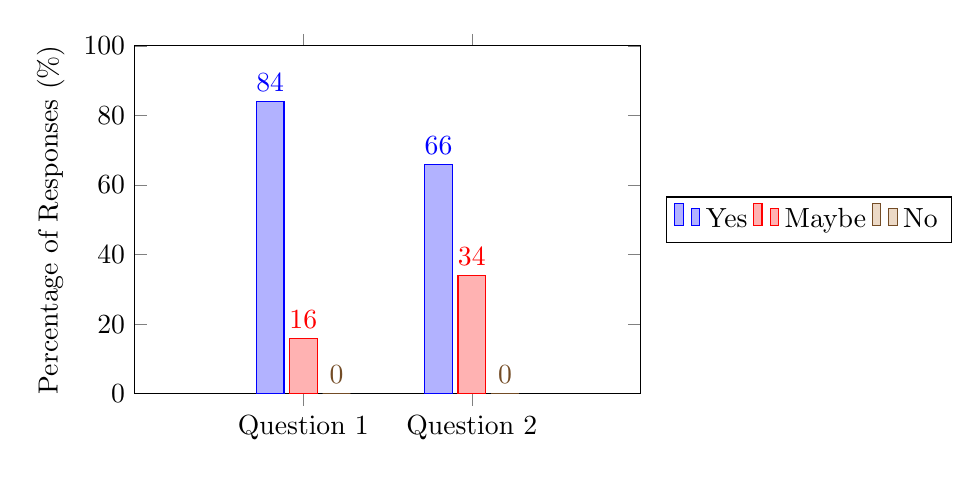
\begin{tikzpicture}  
\begin{axis}  
[  
    ybar,
    width=8cm,
    height=6cm,
    enlarge x limits=1,       
    ylabel={Percentage of Responses (\%)},
    ymin=0,
    ymax=100,
    symbolic x coords={Question 1, Question 2},  
    xtick=data,  
    nodes near coords,  
    nodes near coords align={vertical},  
    legend style={at={(1.05,0.5)},anchor=west, legend columns=-1},
    ]  
\addplot coordinates {(Question 1, 84) (Question 2, 66)};
\addplot coordinates {(Question 1, 16) (Question 2, 34)}; 
\addplot coordinates {(Question 1, 0) (Question 2, 0)}; 
\legend{Yes, Maybe, No}  
  
\end{axis}  
\end{tikzpicture} 
\begin{enumerate}
    \item After using the app are you interested in the concept?
    \item Would you potentially use such an app?
\end{enumerate}
\caption{Combined results of concluding questions}
\label{fig:conclAns}
\end{figure}
\FloatBarrier

\subsection{System Usability Scale (SUS)}
The system usability scale was completed by 8 participants during the in person evaluation, after the user had completed all of the tasks. Calculating the SUS score involves subtracting 1 from the responses to the positively worded questions, then, responses to the negatively worded questions are subtracted from 5. These values are then summed together, and multiplied by 2.5 to give a SUS score in the range 0-100. The participant responses to each question, and, corresponding SUS score are shown in \ref{appendix:susQns}. The average SUS score derived from all responses is 84.38, obtaining the highest grade of A+ according to the grading scale proposed by James Lewis and Jeff Sauro \cite{susGrades}. These results are a reliable measure of system usability, portraying how participants were impressed by the usability of the application.

\subsection{Online Evaluation Questions}

The online evaluation was completed by 24 participants after viewing the videos, and, screenshots of the application. All questions were answered through a five point Likert scale ranging from 1 being a very positive response, to 5 being a very negative response. This applies to all questions except question 4 in the general question section where the scale is reversed. The first video introduced the application, this covered creating profiles, customizing profiles, and , the adding of friends. The responses to this video were very positive with most participants responding that the application looked very easy to navigate, the design was very consistent, and, there was a sufficient level of customisation for profiles, shown by average responses ranging from 1 to 1.5. The second video showcased the creation, customisation, and, general usage of groups. Participants again responded positively stating that the processes shown looked very easy to perform, the design was very consistent, and, the level of customisation for groups was sufficient, with average responses ranging from 1.21 to 1.42. The general question section was answered with respect to the videos watched, and, the screenshots presented. Again, participant responses were very positive with participants liking the consistent design, and, thinking that the application seemed easy to use, navigate, and, learn. The average responses are shown below with a full table of responses at \ref{appendix:onlineQnResp}.

\begin{table}[!ht]
    \centering
    \begin{tabular}{|l|l|l||l|l|l||l|l|l|l|}
    \hline
    \multicolumn{10}{|c|}{Average Response } \\
    \hline
     \multicolumn{3}{|c||}{Video 1 } &
     \multicolumn{3}{|c||}{Video 2 } &
     \multicolumn{4}{|c|}{General } \\
    \hline
        \textbf{a} & \textbf{b} & \textbf{c} & \textbf{a} & \textbf{b} & \textbf{c} & \textbf{1} & \textbf{2} & \textbf{3} & \textbf{4} \\ \hline
    \hline
        1.50 & 1.29 & 1.50 & 1.42 & 1.21 & 1.33 & 1.75 & 1.42 & 1.25 & 4.58 \\ \hline
    \end{tabular}
\end{table}

\subsection{Participant Feedback}

Throughout both evaluations there was multiple opportunities to give textual feedback regarding the application. These free text responses have been split into two categories, application feedback, and, suggested improvements. Some examples from both categories are listed below.
\vskip\baselineskip
\textbf{Application Feedback:}
\begin{itemize}
    \item "The app was very clean and crisp, while also looking easy to navigate through and use for multiple age ranges."
    \item "The design was consistent and used formats that are recognisable to the common user which is good because it utilises formats that the user already knows how to use."
    \item "Great customisation options. Improves user experience"
    \item "Just minor things about the app like loading states \& feedbacks. A lot of Nielson's heuristics are respected!"
    \item "I think this app would be very useful and believe that it would be popular with young people and I know that I would use it along with my friends"
    \item "Colours worked well together and was a very easy to learn system"
\end{itemize}
\vskip\baselineskip
In general, participants were very pleased with the application with many liking the consistent design and ease of use. The use of recognised design patterns and attempts to increase usability were noted by participants, this was excellent feedback to receive.   
\vskip\baselineskip
\textbf{Suggested Improvements:}
\begin{itemize}
    \item "When registering, users should be logged in automatically; rather than putting in their details again"
    \item "Possible light/dark mode toggle"
    \item "As an alternative to the clock, clicking show members could show a list of statuses. This would be useful in case of a large number in a group."
    \item "The ability to change the background colour from purple."
    \item  "In general I think it's a really cool idea for an app, but I wonder if in practice people using it would remember to change their status regularly to update their friends on their whereabouts. Perhaps some notifications could work well here. "
\end{itemize}
\vskip\baselineskip
There were many improvements suggested by participants which are invaluable, this presents new ideas, and, feature that could be implemented in future iterations, improving the application. Some noticeable feedback was that users would like the ability to change theme colours and have light and dark mode toggles. This was a wont have requirement listed in \ref{non-functional}, so although this release did not have this feature due to being limited by time constraints, this was a feature that could be implemented in the future. Integration with push notifications was also mentioned by participants, this was another feature listed (see \ref{functional}) that unfortunately could not be implemented in this release, but hopefully in the future. Other suggestions such as  automatic logins, and, listing of member statuses were new ideas that could now be considered for a future release.

\subsection{In Person Experiment Observations}

As the in person evaluation was observed, some extra insight was gained into how users were interacting with the application, and completing tasks. Behaviour was noted that was previously not seen, or, considered during the implementation, and, testing of the application.
\vskip\baselineskip
\textbf{Observed Behaviour:}
\begin{enumerate}
    \item When asked to register for an account, majority of participants would enter text into the sign in form and not realise they had to press the register button first.
    \item When asked to find their friends list, a few participants did not find the icon representing the friends list screen significant, and, struggled to navigate to this screen.
\end{enumerate}

\textbf{Potential Solutions:}
\begin{enumerate}
    \item A screen could be presented to the user that has clear sign in, and, register buttons before corresponding forms are presented to the user. 
    \item A text label below the friends list icon could be added to help users recognise how they are to access this screen.
\end{enumerate}
\vskip\baselineskip

\section{Summary}
